% !TeX root = ../main.tex
% Add the above to each chapter to make compiling the PDF easier in some editors.

\chapter{Evaluation}\label{chapter:evaluation}

This chapter evaluates the proposed permutation-planning and execution pipeline. We describe the experimental methodology, detail the hardware and software configuration used for the measurements, and present quantitative results for runtime, peak memory usage, and memory movement that compare the baseline and optimized strategies.

\section{Setup}

All experiments reported in this chapter were executed on a single central machine dedicated to benchmarking and performance validation. The machine is built around a 12th-generation Intel Core i5 processor in specific the 12th Gen Intel(R) Core(TM) i5-12450H, and was configured to expose the AVX2 instruction set. The system used 16~GB of main memory for every run reported here. Kernel generation and compilation were performed using the GNU compiler version 11.4.0, and the specific \ac{TCCG} instance as pf v0.1.1. Experiments targeted double precision arithmetic and relied on a conservative generator setting of \texttt{maxImplementations = 1} to ensure stable and comparable kernels across runs.

Parallel execution was driven by the GNU OpenMP runtime and controlled through the environment affinity hints stored alongside the generator configuration \newline\texttt{GOMP\_CPU\_AFFINITY=0-12}. On this machine the measured core topology presented eight logical cores and twelve virtual cores; accordingly the affinity and thread settings were explicitly adjusted to make the runtime parallelism unambiguous. To validate portability and to check for operating-system-level effects, the same experiments were also executed on Windows Subsystem for Linux 2 (WSL2) running Ubuntu 22.04.

\section{Impact of ignoring the largest intermediate tensor}

The first empirical study was designed to evaluate the central hypothesis of this work that intentionally avoiding permutations for the largest intermediate tensors in a contraction sequence can reduce the overall peak and intermediate memory requirements without compromising the local contraction choices. To test this hypothesis at scale we generated a corpus of 5,200 random tensor networks with between seven and twenty tensors each and compared two execution strategies. The first strategy is a conservative baseline that always applies the locally optimal permutation for each contraction. The second strategy freezes the single largest intermediate tensor ($k$ = 1) and therefore does not permute it prior to contractions. For both strategies we measured the peak resident memory and the summed intermediate memory movement produced during the complete contraction.

Figure~\ref{fig:ignore_largest_5200} displays the aggregated results. The figure summarises the relative difference between the baseline and the ignore-largest strategy. Across the whole corpus the ignore-largest strategy produced a substantial reduction in measured memory. On average the peak and intermediate memory usage was lower by approximately 45\% when the largest intermediate tensor was left unpermuted. Moreover, the benefit is not uniform across network sizes. As network size increases (more tensors per network) the effect becomes more pronounced, reflecting the intuition that larger contraction trees increasingly channel data movement through a small set of large intermediates that act as choke points. In these cases avoiding permutations on the dominant intermediate relieves the most significant memory-traffic hotspot and therefore yields larger savings.

These results support the claim that treating layout for the largest intermediate tensors as a first-class design choice can deliver practical memory reductions in realistic contraction workloads. The remainder of this chapter examines representative individual networks from the corpus, quantifies variance and outliers, and investigates how the observed savings depend on rank distributions and contraction topologies.

\begin{figure}[ht]
	\centering
	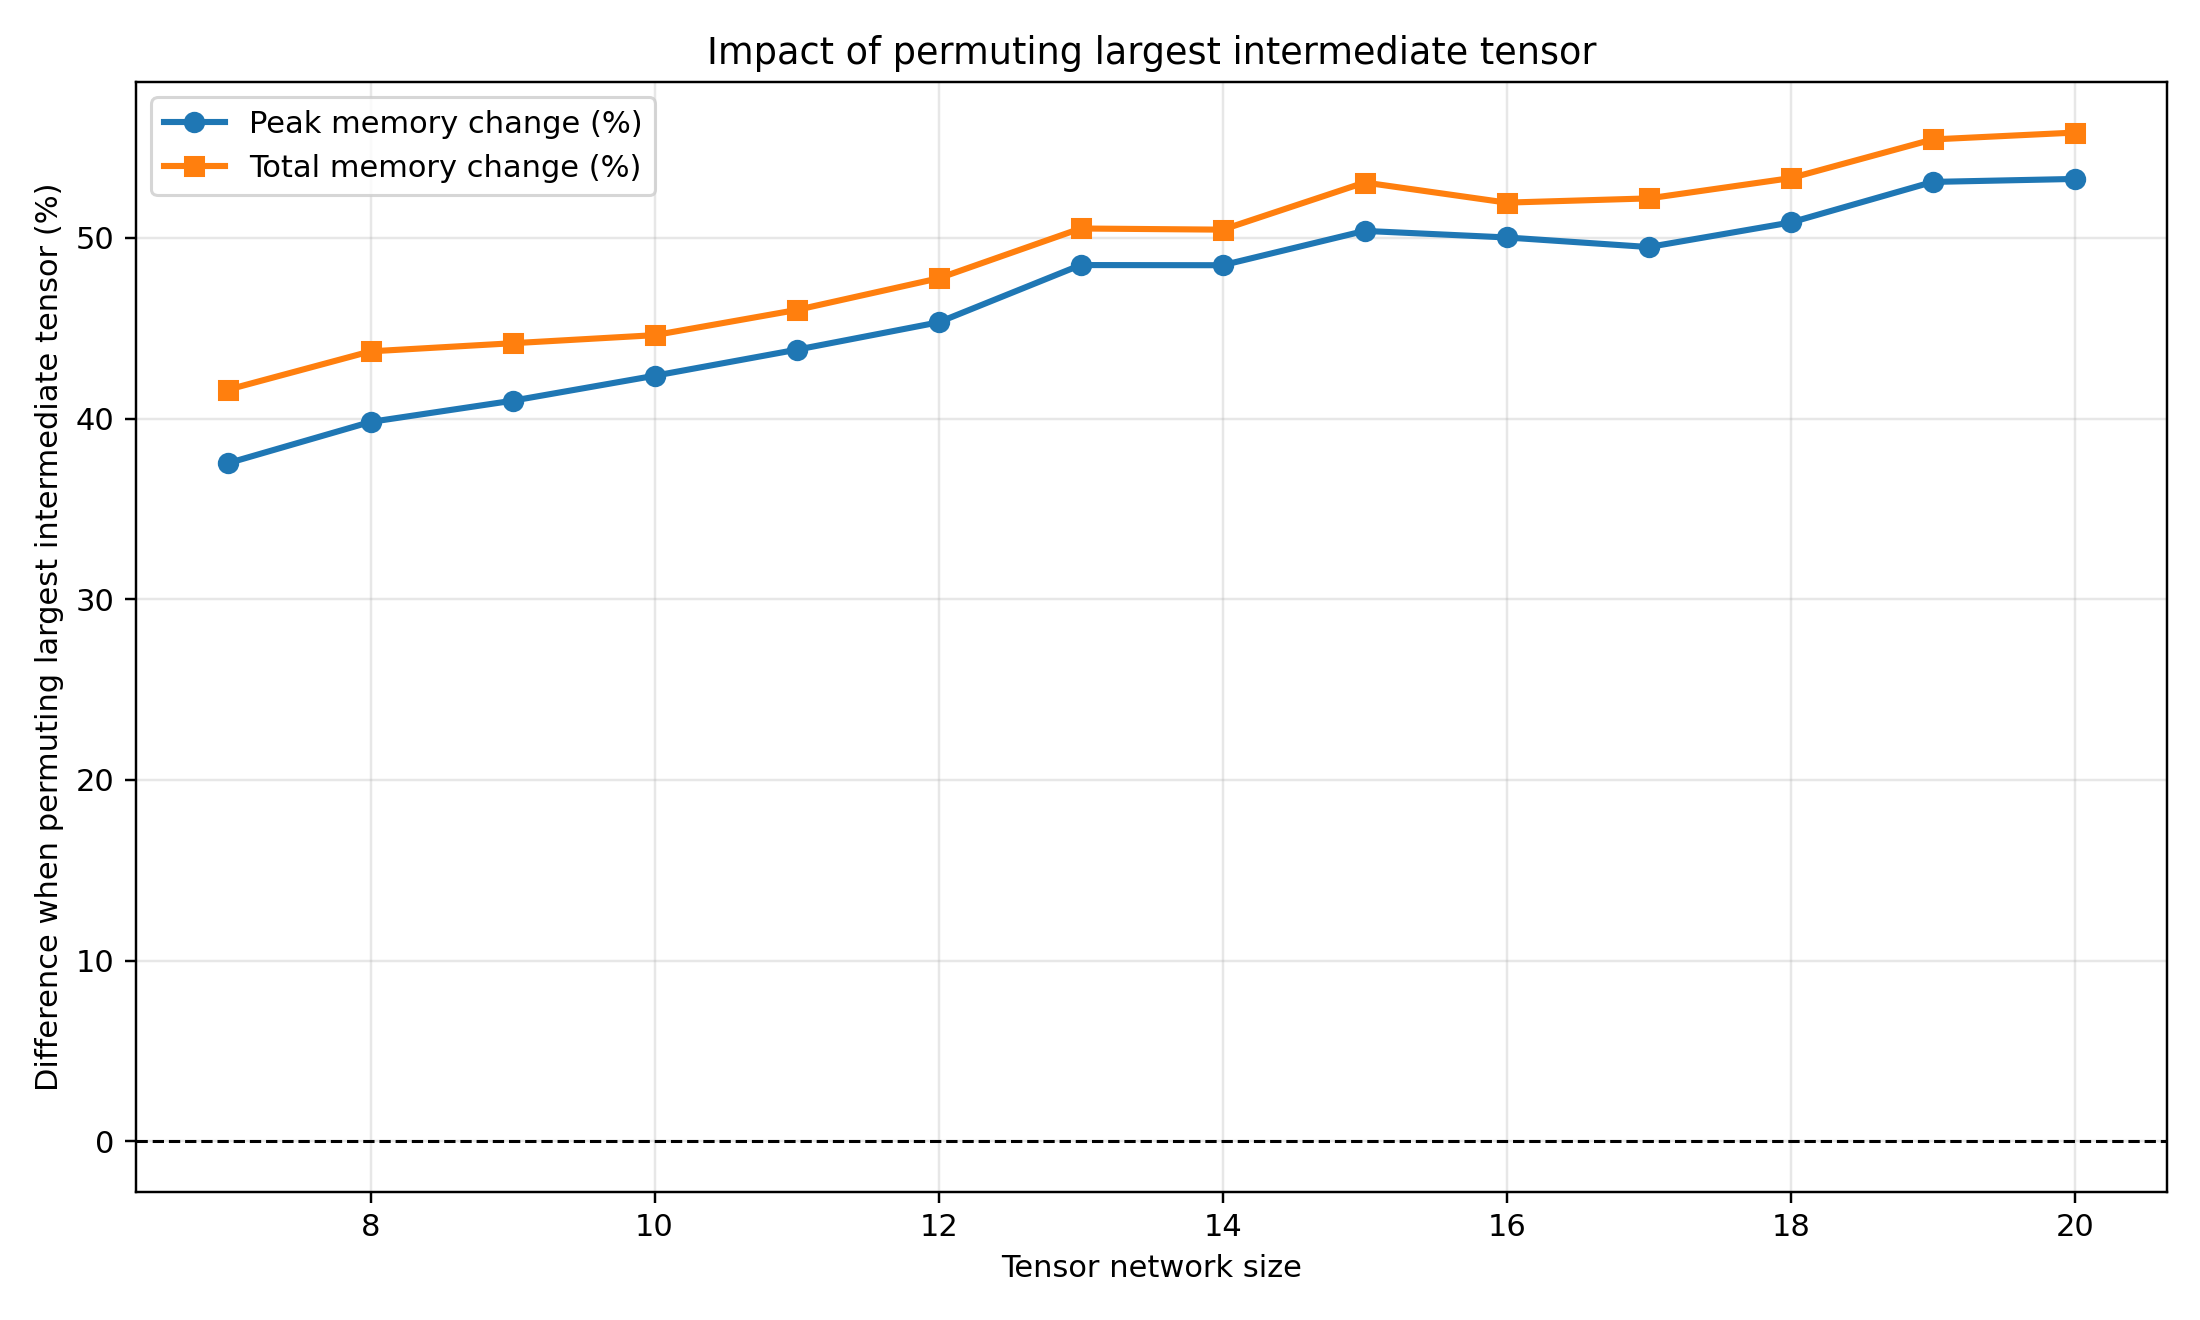
\includegraphics[width=0.9\textwidth]{figures/5200_impact_of_ignoring_largest_intermediate_tensor.png}
	\caption{Impact of ignoring permutation of the largest intermediate tensor on peak and intermediate memory.}
	\label{fig:ignore_largest_5200}
\end{figure}

